\subsection{Navigasjon}
Appen består av to hovedelementer for navigasjon, et bottom-navigation element, og et navigation-drawer element. I tillegg til disse har den en swipe-funksjon når man befinner seg i forsiden, kartsiden og vennesiden. Det vil være mulig å navigere mellom disse tre sidene med bottom-navigation elementet, men også å swipe fra venstre til høyre og motsatt. Tilgjengelig fra de fleste sider vil være en navigation-drawer som brukes til å navigere til resten av appen.

Grunnen til denne oppdelingen er for å skille mellom sider som blir brukt mye og sider som blir brukt lite. Vi har valgt å bruke bottom-navigation og swipe-funksjonen til forsiden, kartsiden og vennesiden, fordi de er sentrale og brukes nesten hver gang appen er i bruk. Forsiden er det samme som oversiktssiden, så dette vil være landingssiden når brukeren logger inn. I navigation-drawer elementet kan man blant annet navigere seg til innstillinger og enhetskatalogen.

\subsubsection{Flyt}

\begin{figure}[H]
    \centering
    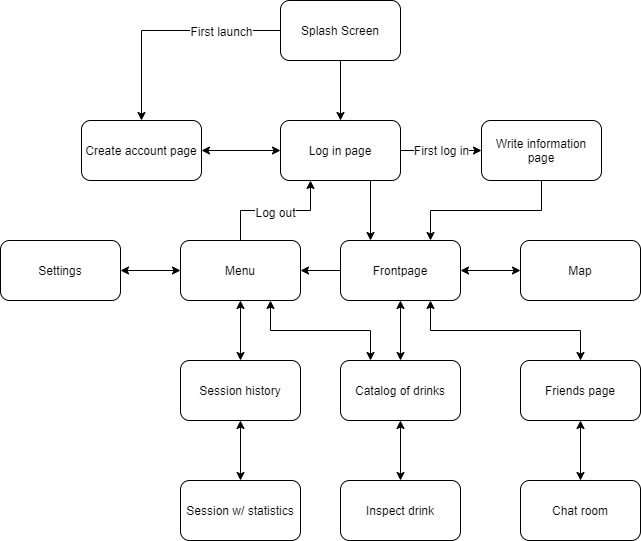
\includegraphics[scale=0.5]{images/lille_promille_float_diagram.drawio.png}
    \caption{Skisse som viser hvor man kan navigere seg til fra hvilke sider i appen.}
\end{figure}

\subsubsection{Navigation Pattern}
Bla bla bla

\subsection{Teknisk oppbygging}
Blablabla

\subsubsection{Lagring og uthenting av data}
For å lagre brukerdata benyttes Firestore. Dette gjøres via Firebase, her lagres brukere i en "user" collection. Hver bruker lagres med en UUID som autogeneres fra Firebase. 

Brukerinformasjonen lagres rett i dokumentet til brukeren, mens enhetskatalogen og økt historikken lagres i collections på brukeren. 
Disse 

\subsubsection{Brukerhåndtering}
Håndtering av brukere gjøres gjennom Firebase.

\section{Ressurser}
\subsection{Services}


\subsection{Fragmenter}

\subsection{Bilder}
Bilder i appen vil bestå for det meste av ikoner, samt noen iterasjon 

\subsection{Biblioteker}
\subsubsection{Firebase}